\documentclass[9pt]{beamer}
\usepackage{minted}
%\usemintedstyle{manni}
\usemintedstyle{murphy}
\usepackage{hyperref}
\hypersetup{
colorlinks=true,
urlcolor=blue
}
\usepackage{graphicx}

\begin{document}
\title{h5py}
\author{Nick Thompson} 
\date{\today}

\frame{\titlepage}

\begin{frame}[fragile]
\frametitle{Getting started:}
\begin{minted}{bash}
$ git clone https://github.com/NAThompson/h5py_talk.git
$ cd h5py_talk
$ sudo /bin/bash
$ docker run -it -v `pwd`:/hdf5_talk /bin/bash
\end{minted}
\end{frame}

\begin{frame}[fragile]
  \frametitle{What is the best scientific data format?}
  \pause
  Compressed CSV.
\end{frame}


\begin{frame}[fragile]
  \frametitle{What is the second best scientific data format?}
  HDF5.
\end{frame}

\begin{frame}[fragile]
  \frametitle{Ever had this conversation?}
  \begin{itemize}
  \item ``These ascii files are too large.''
  \item ``We could use binary.''
  \item ``How long will that take?''
  \item ``4 hours.''
  \item (3 years later . . .) ``WTF!!!''
  \end{itemize}
\end{frame}

\begin{frame}[fragile]
  \frametitle{Edict:}

  Anyone who introduces a custom binary format shall be hanged.
\end{frame}

\begin{frame}[fragile]
  \frametitle{Where can I use my HDF5 files?}
  \begin{itemize}
  \item Fortran, C, C++, Java, Python, Octave, Matlab, IDL, LabView
  \end{itemize}
\end{frame}


\begin{frame}[fragile]
  \frametitle{Example:}

  \begin{minted}{bash}
    $ hdfview example_files/compound.h5
  \end{minted}
  \begin{figure}
    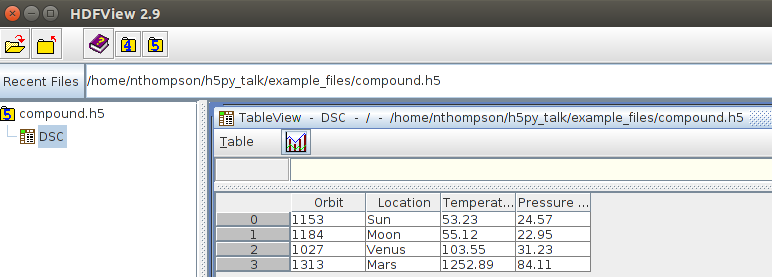
\includegraphics[scale=0.3]{fig/hdfview.png}
  \end{figure}
  \pause
  If you are attempting this in the Docker image, you'll need to set up X-window forwarding.
\end{frame}

\begin{frame}[fragile]
  \frametitle{Explore HDF5 Files}
  \begin{minted}{bash}
    $ h5ls example_files/compound.h5
    $ h5dump example_files/compound.h5
  \end{minted}
\end{frame}

\begin{frame}[fragile]
  \frametitle{New Visualization Tool:}
  \begin{minted}{bash}
    $ git clone https://github.com/HDFGroup/hdf-compass.git
    $ cd hdf-compass
    $ python HDFCompass.py
  \end{minted}
\end{frame}


\begin{frame}[fragile]
\frametitle{First HDF5 File}
\begin{minted}{python}
>>> import h5py
>>> import numpy as np
>>> f = h5py.File('stock_prices.hdf5')
v>>> f['/stock_prices/DJIA/MMM'] = np.random.random(2048)
>>> f['/stock_prices/DJIA/MMM'].attrs['sample_rate'] = 1
>>> f['/stock_prices/NASDAQ/MU'] = np.random.random(2048)
>>> f['/stock_prices/NASDAQ/MU'].attrs['sample_rate'] = 1
>>> f.close()
\end{minted}
\end{frame}

\begin{frame}[fragile]
  \frametitle{Analyzing HDF5 file}
  \begin{minted}{python}
    >>> import h5py
    >>> f = h5py.File('stock_prices.hdf5', 'r')
    >>> [key for key in f.keys() ]
    >>> ['stock_prices']
    >>> list(f.keys())
  \end{minted}
  \pause
  Use a callback to get more details:
  \begin{minted}{python}
    >>> def print_attrs(name, obj):
    >>>     print(name)
    >>>
    >>> f.visititems(print_attrs)
    >>>
    >>> def p(name):
    >>>     print(name)
    >>>
    >>> f.visit(p)
  \end{minted}
\end{frame}

\begin{frame}[fragile]
  \frametitle{Standards Built on Top of HDF5}
  Once you agree on a set of groups and attributes, you can create standards on top of HDF5:
  \begin{itemize}
  \item NetCDF (for climatology, meteorology, GIS)
  \item PH5 (seismology)
  \item 
  \end{itemize}
\end{frame}

\begin{frame}[fragile]
  \frametitle{Within-Dataset Compression}
  Normally compressing data \emph{within} a file is unforgivable, but HDF5 makes it transparent:
  \begin{minted}{bash}
    >>> import h5py
    >>> import numpy
    >>> f = h5py.File('compressed.hdf5')
    >>> zipped_dst = f.create_dataset('ones', shape=(4096,), dtype='int32', compression='gzip')
    >>> zipped_dst = np.ones(4096)
    >>> f.close()
    >>> g = h5py.File('compressed.hdf5', 'r')
    >>> dst = g['ones']
    >>> a = dst[:]
    >>> len(a)
        4096
  \end{minted}
\end{frame}

\begin{frame}
  \frametitle{}
\end{frame}

\end{document}
